\documentclass{beamer}
\usetheme{Boadilla}

\usepackage{graphicx}
\usepackage{amsmath}
\usepackage{hyperref}

\title{CNNs for Image Processing}
\author{Yashwant Bhosale}
\institute{COEP Tech.}
\date{\today}

\begin{document}

\maketitle

\section{Section 1}
\subsection{sub a}

\begin{frame}
    \frametitle{Handwritten Digit Recognition}
    \begin{center}
        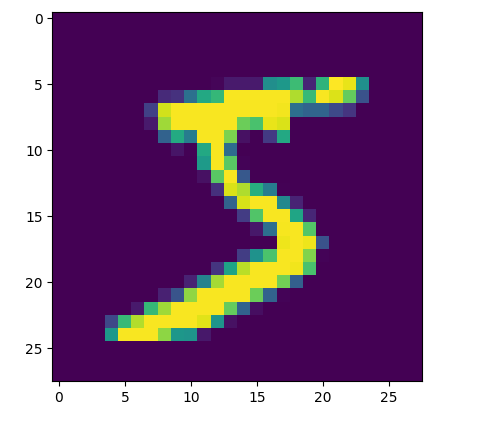
\includegraphics[width=5cm]{Screenshot from 2025-02-03 14-53-39.png}
    \end{center}
    Have you ever wondered how computers can recognize handwritten digits? and given a program that recognizes handwritten digits, can it draw those?
\end{frame}

\begin{frame}
    \frametitle{How can humans do this so effortlessly?}

    \begin{enumerate}
        \item Our brains have evolved to be incredibly adept at visual pattern recognition,
    
        \item Humans learn to recognize digits through exposure to a variety of handwriting samples over time, while NNs require large, labeled datasets to train and learn features automatically. 

        \item Humans can easily adapt to different handwriting styles, interpret ambiguous digits based on context, and recognize digits even if they are slightly distorted or rotated, whereas NNs might struggle with such variations unless specifically trained on diverse data. 

    \end{enumerate}
    
\end{frame}

\begin{frame}
    \frametitle{But, what is NN?}

    \begin{center}
        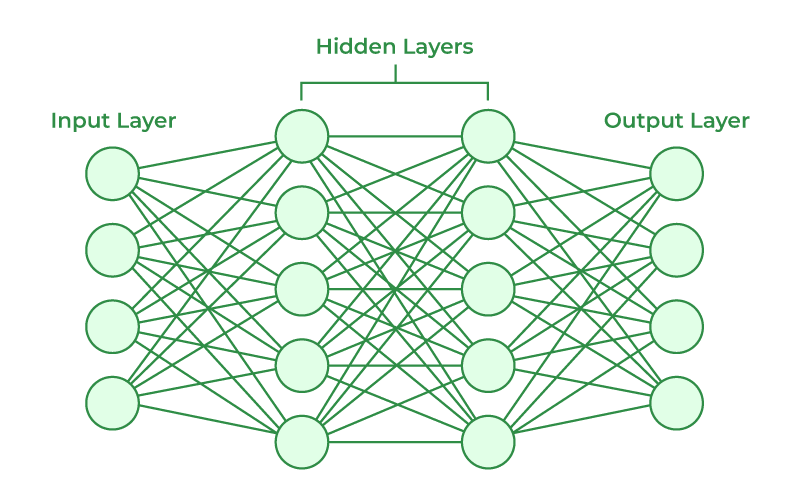
\includegraphics[width=7cm]{Neural-Networks-Architecture.png}
    \end{center}
    
    NN means \textbf{Neural Networks}
    \\
    As the name suggests there are \textbf{Neurons} in the neural network.
    \\
    and there are \textbf{layers} of these \textbf{neurons}.
    \\
    In a bird's eye view, there are 3 types of layers: \textbf{input layer}, \textbf{hidden layer} and \textbf{output layer}
\end{frame}

\begin{frame}
    \frametitle{Why does network of neurons behave intelligently?}
    \begin{center}
        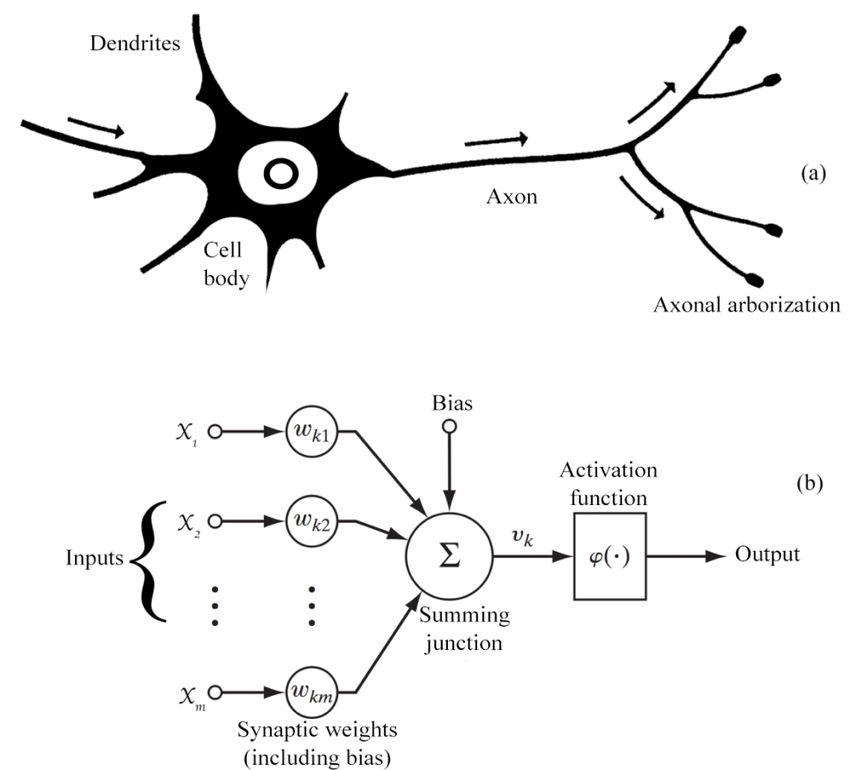
\includegraphics[width=5cm]{neural-netork-weights-biases.png}
    \end{center}
    Neural networks appear "intelligent" because they can learn and adapt to complex patterns in data by adjusting internal parameters \textbf{(weights and biases)} through a process called \textbf{backpropagation}, effectively \textcolor{red}{mimicking the way the human brain learns by making connections between neurons based on experience}, allowing them to make predictions and classifications on new data with a high degree of accuracy, especially when dealing with non-linear relationships between inputs and output
\end{frame}

\begin{frame}
    \frametitle{Math behind Neural Networks}
    \textbf{Linear Transformation}
    \\
    In a neural network, we have layers of neurons. Each neuron is connected to the neurons in the previous layer through weighted connections. Mathematically, this connection can be represented as:
    \[Z  = W \cdot X + b\]
    \begin{itemize}
        \item \(Z\) is the linear combination of inputs \(X\), weights \(W\), and bias \(b\).
        \item  \(W\)  represents the weights associated with each connection.
        \item \(X\) is the input data
        \item \(b\) is the bias term
    \end{itemize}   
\end{frame}

\begin{frame}
    \frametitle{Math behind Neural Networks}
    \textbf{Activation Function}
    \\
    The output of a neuron is usually passed through an activation function, which introduces non-linearity to the model. The most commonly used activation functions are:
    \\
    \begin{itemize}
        \item Sigmoid Function:
        \[A= \frac{1}{(1 + e^{-Z})}\]
        \item ReLU (Rectified Linear Unit):
        \[A=max(0, Z)\]
    \end{itemize}
\end{frame}

\begin{frame}
    \frametitle{Math behind Neural Networks}
    \textbf{Loss Function}
    The loss function measures how well the model is performing. For classification tasks like ours, we often use cross-entropy loss
    \[L(y, \hat{y}) = -\sum(y_i * log(\hat{y}_i))\]
    \begin{itemize}
        \item \(y\) is the actual label
        \item \(\hat{y}\) is the predicted label
    \end{itemize}
\end{frame}

\begin{frame}
    \frametitle{Math behind Neural Networks}
        The model learns by minimizing the loss function. Gradient descent is the optimization technique to update the model’s parameters (weights and biases) iteratively.

        \[W_{new} = W_{old} - \eta \cdot \frac{\partial L}{\partial W}\]

        \[b_{new} = b_{old}-\eta \cdot \frac{\partial L}{\partial W}\]

        here \(\eta\) is Learning Rate
\end{frame}

\begin{frame}
    \begin{tabular}{|c|c|c|}
\hline
\textbf{Activation Function} & \textbf{Formula} & \textbf{Range} \\[5px]
\hline
    % I have been asked to link different files/folders using table 
    \href[pdfnewwindow]{run:.main-1.pdf}{main-1.pdf} & \( \sigma(x) = \frac{1}{1 + e^{-x}} \) & (0, 1) \\[5px]
\hline
ReLU & \( f(x) = \max(0, x) \) & [0, \( \infty \)] \\[5px]
\hline
Tanh & \( f(x) = \frac{e^x - e^{-x}}{e^x + e^{-x}} \) & (-1, 1) \\[5px]
\hline
\end{tabular}
    
\end{frame}

\end{document}
